\documentclass[13pt]{article}
\renewcommand{\baselinestretch}{1.2}
\usepackage[utf8]{vietnam}
\usepackage[a4paper, total={6in, 8in}]{geometry}
\usepackage[vietnamese,english]{babel}
\usepackage{hyperref}
\usepackage{mathtools}
\usepackage{amssymb}
\usepackage{indentfirst}
\usepackage{graphicx}
\usepackage{minted}
\usepackage{ragged2e}
\usepackage{multirow}
\usepackage{subcaption}
\usepackage{xurl}
\usepackage{amsmath}
\usepackage{makecell}

\usepackage[hybrid]{markdown}

\renewcommand\theadalign{bc}
\renewcommand\theadfont{\bfseries}
\renewcommand\theadgape{\Gape[4pt]}
\renewcommand\cellgape{\Gape[4pt]}
\usepackage{pbox}

\graphicspath{ {./graphics/} }

\hypersetup{
    colorlinks=true,
    linkcolor=blue,
    citecolor=blue,
    urlcolor=blue,
}

\usepackage[nottoc]{tocbibind}

\begin{document}
\begin{titlepage}
    \begin{center}
        \vspace*{1.8cm}
        \Large
        Distributed System Labwork 3\\
        \Large
        \vspace{0.5cm}
        \begin{center}
            
\includegraphics[scale=1.0]{images/usth_logo1.PNG}
        \end{center}  
        \vspace{0.5cm}
            Group 1 - ICT\\
        \vspace{0.5cm}
            University of Science and Technology of Hanoi\\
        \vspace{0.5cm}
            January, 2022
        \vfill
          
   \end{center}
\end{titlepage}

\newpage
\tableofcontents
\newpage


\section{Introduction}
\subsection{Overview}
\noindent%
MPI(Message Passing Interface) is a library designed to allow users to create programs that can run efficiently on most parallel architectures. In the message-passing model of parallel computation, the processes executing in parallel have separate address spaces. Communication occurs when a portion of one process’s address space is copied into another process’s address space. This operation is cooperative and occurs only when the first process executes a send
operations and the second process executes a receive operation.\cite{MPI Concept}

\noindent%
In this labwork, we try to build a file transfer system using MPI. We will use C in this labwork.


\subsection{Protocol}
\begin{figure}[h]
    \centering
    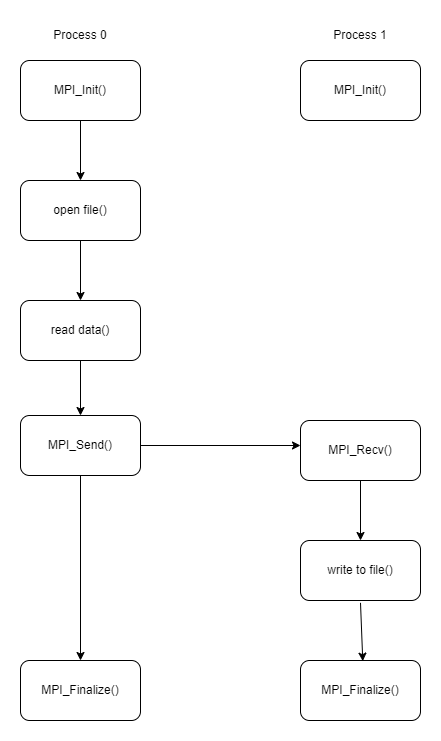
\includegraphics[scale=0.45]{images/mpi.png}
    \caption{Protocol diagram}
    \label{fig:protocol}
\end{figure}

\section{Implementation}
\noindent%
This is the implementation of the labwork. In order to run the file, please type 
"mpicc mpi$\_$ftp.c -o mpi" and then "mpirun -np 2 ./mpi"

\begin{minted}[linenos,tabsize=2,breaklines]{c}
#include <stdio.h>
#include <mpi.h>
#include <string.h>
#include <stdlib.h>
#define MAX_SIZE 1024
#define size_tag 2001
#define char_tag 2002

void send_file(FILE* fp, char* filename, char* buffer, int rank_des) {
	fp = fopen(filename, "r");
	if (fp == NULL) {
		perror("Error in reading file..\n");
		exit(1);
	}
	else {
		printf("Reading file successfully..\n");
	}
	int buffer_size;
	while (1) {
		int buffer_size = fread(buffer, 1, MAX_SIZE, fp);
		MPI_Send(&buffer_size, 1, MPI_INT, rank_des, size_tag, MPI_COMM_WORLD);
		MPI_Send(buffer, buffer_size, MPI_CHAR, rank_des, char_tag, MPI_COMM_WORLD);
		if (buffer_size < MAX_SIZE) {
			printf("\nUpload finished.\n");
			break;
		}
	}
	fclose(fp);

}

void receive_file(FILE* fp, char* filename, char* buffer, int rank_from) {

	fp = fopen(filename, "a");
	if (fp == NULL) {
		perror("Error in reading file..\n");
		exit(1);
	}
	else {
		printf("Reading file received successfully..\n");
	}
	int buffer_size;
	while (1) {
		MPI_Recv(&buffer_size, 1, MPI_INT, rank_from, size_tag, MPI_COMM_WORLD, MPI_STATUS_IGNORE);
		MPI_Recv(buffer, buffer_size, MPI_CHAR, rank_from, char_tag, MPI_COMM_WORLD, MPI_STATUS_IGNORE);
		fwrite(buffer, 1, buffer_size, fp);
		if (buffer_size < MAX_SIZE) {
			printf("\nWrite finished.\n");
			break;
		}
	}
	fclose(fp);
}

int main(int argc, char* argv[]) {
	FILE* fp;
	int my_id, numprocs, len;
	char buffer[MAX_SIZE];
	char name[MPI_MAX_PROCESSOR_NAME];
	int client_to_server = 1;
	MPI_Init(&argc, &argv);

	MPI_Comm_rank(MPI_COMM_WORLD, &my_id);
	MPI_Comm_size(MPI_COMM_WORLD, &numprocs);

	if (numprocs < 2) {
		printf("Need at least 2 processes");
	}
	MPI_Get_processor_name(name, &len);
	char* root_send = "send.txt";
	char* slave_received = "received.txt";
	memset(&buffer, 0, sizeof(buffer));
	if (client_to_server) {
		if (my_id == 0) {
			send_file(fp, root_send, buffer, 1);
		}
		else if (my_id == 1) {
			receive_file(fp, slave_received, buffer, 0);
		}
	}
	else {
		if (my_id == 0) {
			receive_file(fp, root_send, buffer, 1);
		}
		else if (my_id == 1) {
			send_file(fp, slave_received, buffer, 0);
		}
	}
	MPI_Finalize();
}
\end{minted}

\noindent%
This is the result:
\begin{figure}[H]
    \centering
    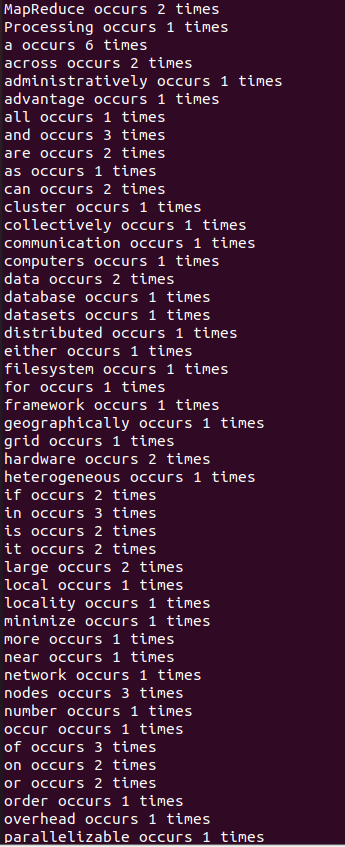
\includegraphics[scale=1.0]{images/result.PNG}
    \caption{Result after file transfer}
\end{figure}


\section{Contribution}
\begin{table}[ht!]
  \begin{center}
    \begin{tabular}{|l|l|}
      \hline
      \textbf{Member} & \textbf{Contribution}\\
      \hline
      Nguyen Xuan Tung & Send fIle code\\
      \hline
      Nguyen Quang Anh & Receive file code\\
      \hline
      Lu Khanh Huyen & Design Protocol\\
      \hline
      Tran Hong Quan & MPI concept\\
      \hline
      Vu Duc Chinh & Report\\
      \hline
    \end{tabular}
    \caption{Contribution Table}
  \end{center}
\end{table}

\begin{thebibliography}{9}
\bibitem{MPI Concept}
William Gropp, Ewing Lusk, and Anthony Skjellum. 2014. Using MPI: Portable Parallel Programming with the Message-Passing Interface. The MIT Press.
\end{thebibliography}

\end{document}
